\section{Off Policy Actor Critic}
The first actor-critic algorithm we examined, presented in Algorithm \ref{general_actor_critic},
is a fully on-policy method. This approach has significant drawbacks, as we discussed in the policy
gradient chapter. Training samples are collected based on the current policy-the very policy we aim
to optimize. As a result, after each gradient update, we can no longer use the previously collected
samples. If the method were off-policy, we could achieve better sample efficiency and enhanced
exploration by following a variety of different policies. This concept will be further explored in the 
following section.
\subsection{First Attempt}
The first idea that comes to mind for making the algorithm off-policy is to introduce a replay buffer,
similar to what we did in the DQN section, resulting in an approach like this:
\begin{algorithm}[H]
  \large
    \caption{}\label{first_off_policy_attempt_act_crit}
    \begin{algorithmic}
        \STATE Init. $s,\theta,w, D = \{\}$
        \FOR{$t=0,1,\dots,T$}
        \STATE sample $a_t \sim \pi_{\theta}(s_t)$
        \STATE sample $s_{t+1} \sim P(s_{t+1}|s_t,a_t)$ and  $r_{t+1} \sim R(s_t,a_t)$
        \STATE store $(s_t,a_t,s_{t+1},r_{t+1})$ in $D$
        \STATE sample a batch $((s_i,a_i,s_{i+1},r_{i+1}))$ from buffer $D$
        \STATE execute Actor Critic Algorithm \ref{general_actor_critic} on batch
        \ENDFOR
    \end{algorithmic}
\end{algorithm}
However, the algorithm has some significant flaws and cannot be used as it is currently written. There are two 
main issues. 
\paragraph{Value Function} The first concerns the target values
$$y_i = r_{i+1} + \gamma V^\pi_{w}(s_{i+1})$$
These targets are incorrect because the batch samples come from older actors, yet we use them to compute target values for 
training the current critic. As a result, the current actor is being guided by targets that reflect outdated policies, rather 
than its own behaviour.\newline 
To address this issue, we will learn the Q-value function instead of the V-function.  Recall that the Q-function represents 
the expected return starting from a given state, taking a specific action, and then following the policy thereafter. Using the 
relationship between the value function and the Q-function given in Equation \eqref{eq:v_to_q}, we can rewrite the target as:
\begin{align*}
    y_i = r_{i+1} + \gamma V^\pi_{w}(s_{i+1}) 
    &=  r_{i+1} + \gamma Q^\pi_{w}(s_{i+1},a') \qquad a' \sim \pi_\theta(\cdot|s_i)
\end{align*}
This allows us to reuse  $s_{t+1}$ from the replay buffer, while sampling the corresponding action $a'$ from the current 
policy. In doing so, our target values remain aligned with the actor's present behaviour. If we had insisted on using the 
value function in an off-policy setting, we would have needed to invoke the simulator to generate the actions the actor would 
take and observe the resulting next states—an expensive and impractical process. In contrast, with this Q-function approach, 
we only need to sample $a'$ from the current policy, which is straightforward since the policy is represented by a neural 
network. Thus, the procedure remains both accurate and efficient.

\paragraph{Policy Gradient} The second problem is that the policy gradient is defined as an expectation over the current 
policy, as seen in Equation \ref{polygrad_td}. This implies that we cannot directly use the samples from the batch. 
We’ve previously discussed how to mitigate this using importance sampling, but another option is to simply
sample again from the current actor, resulting in:
$$\nabla_\theta J(\theta) \approx \nabla_\theta \log{\pi(a_i^\pi|s_i)A^\pi(s_i,a_i^\pi)} \qquad a_i^\pi \sim \pi_\theta(\cdot|s_i) (\text{current actor})$$
%This approach remains efficient, as sampling is quick.\newline\newline 
While some parts of what we have looked at here may seem a bit incoherent/random, I believe this explanation helps to 
understand state of the art off-policy actor-critic methods. These methods are quite similar to what we've discussed here,
so by the time we look at them next, it should feel more familiar when reading the code for these algorithms. 
That’s the goal, at least! As a reminder, policy gradients don't have to be defined solely through the 
advantage function; they can also be defined directly using the Q-function removing the need to also learn a V-function.


%Off-Policy Actor-critics methods have the following structure:
%\begin{enumerate}
%    \item Update critic $Q_\phi(s,a)$ for current policy (arbitrary stochastic behaviour policy not the optimal policy) using off-policy data
%    \item update the actor $\pi_\theta(a|s)$ \begin{itemize}
%        \item stochastic updates: Traditional methods
%        \item deterministic updates: DDPG,TD3
%        \item variational update: SAC
%    \end{itemize}
%\end{enumerate}

\subsection{Updating the critic}
There are multiple ways to update the critic (see Section \ref{section:td-methods} for details) but in most cases, the update 
resembles the approach used in DQN.\newline 
In contrast, there are several different strategies for updating the actor, which we will explore next.

%\subsection{Updating the actor}

%\subsubsection{Stochastic  updates}
%Stochastic updates are among the simplest methods. In this approach, the 
%objective and its gradient are given by:
%$$  J(\theta) = \mathbb{E}_{(s,a)\sim \pi_\theta(a|s)}[A^\pi(s,a)] 
%=  \mathbb{E}_{(s,a)\sim \pi_\theta(a|s)}[Q^\pi(s,a)-V^\pi(s)]$$
%The gradient of the objective is:
%$$ \nabla_\theta J(\theta) =  \mathbb{E}_{(s,a)\sim \pi_\theta(a|s)}
%[\nabla_\theta\log{\pi_\theta(a|s)}\left(Q^\pi(s,a)-V^\pi
%(s)\right)]$$
%The idea here is that we only learn the Value-Function $V$ since we can express the 
%$Q$-Function in terms of it.
%However, this method faces challenges, such as the potential for 
%exploration to collapse too quickly. Additionally, it requires an 
%accurate value function, making the approach more complex.

\subsection{Deterministic updates}
In methods described above, the policy is always modelled as a stochastic policy $\pi(a|s)$. 
Deterministic policy gradient (DPG) instead models the policy as a deterministic decision $a = \pi(s)$.
With this policy the objective of the actor is given by 
$$\max\limits_\theta \underset{s\sim \mathcal{D}}{\mathbb{E}}[Q_\phi(s,\pi_\theta(s))]$$
The gradient of this with respect to $\theta$ is given by
\begin{align*}
\nabla_\theta  \underset{s\sim \mathcal{D}}{\mathbb{E}}[Q_\phi(s,\pi_\theta(s))]
&=  \underset{s\sim \mathcal{D}}{\mathbb{E}}[\nabla_\theta Q_\phi(s,\pi_\theta(s))] \\
&=  \underset{s\sim \mathcal{D}}{\mathbb{E}}\left[ \nabla_a Q_\phi(s,a) \nabla_\theta \pi_\theta(s)|_{a=\pi_\theta(s)}\right]
\end{align*}
At first glance, this may not seem like the policy gradient we derived in the policy gradient chapter. 
However, the deterministic policy gradient is actually a special case of the stochastic policy gradient. 
The proof can be found in \cite{10.5555/3044805.3044850}(Section 3.3).

\subsubsection{Deep Deterministic Policy Gradient (DDPG)} 
DDPG \cite{lillicrap2019continuouscontroldeepreinforcement} is essentially a combination of the deterministic policy
gradient method and DQN, with DQN being used to train the critic. It makes use of the replay buffer and employs the technique 
of using an additional target network for more stable training. The calculation of the max in the target values is addressed 
by using a policy network to compute an action that approximately maximizes the Q-function. Since the policy is deterministic, 
exploration is limited. To encourage better exploration, noise is added to the deterministic policy. 
(see algorithm \ref{algo:ddpg})\newline 
But unfortunately DDPG is quite unstable and requires carefully chosen hyper-parameters. 
Some solutions to this are given with the SAC and TD3 algorithms which we will be looking at in the following.

\subsubsection{Twin Delayed Deep Deterministic (TD3)}
One of the problems with DDPG is that it suffers from overestimation in the learned 
Q-Function. This then leads to the policy breaking, because it exploits the errors 
in the Q-function. Twin Delayed DDPG (TD3) \cite{fujimoto2018addressingfunctionapproximationerror}
is an algorithm (see \ref{algo:TD3}) that addresses this issue by introducing three changes to the original DDPG algorithm.
 \begin{enumerate}
    \item \textbf{Double-Q Learning:} learns two Q-functions instead of one (hence “twin”), and uses
    the smaller of the two Q-values to form the targets in the Bellman error loss functions. 
    Meaning we have critics $(Q_{\phi_1},Q_{\phi_2})$
    \item \textbf{Delayed Policy Updates:} update the policy (and target networks) less frequently than the Q-function.
    \item \textbf{Target Policy Smoothing:} add noise to the target action, to make it harder for the policy to exploit
    Q-function errors by smoothing out Q along changes in action.
 \end{enumerate}

\begin{algorithm}[H]
  \caption{DDPG algorithm from \cite{lillicrap2019continuouscontroldeepreinforcement}\label{algo:ddpg}}
  \begin{algorithmic}
    \STATE Randomly initialize critic network $Q(s, a | \theta^Q)$ and actor
    $\mu(s | \theta^{\mu})$ with weights $\theta^{Q}$ and $\theta^{\mu}$.
    \STATE Initialize target network $Q'$ and $\mu'$ with weights $\theta^{Q'}
    \leftarrow \theta^{Q}$, $\theta^{\mu'} \leftarrow \theta^{\mu}$
    \STATE Initialize replay buffer $R$
    \FOR{episode = 1, M}
      \STATE Initialize a random process $\mathcal{N}$ for action
      exploration
      \STATE Receive initial observation state $s_1$
      \FOR{t = 1, T}
        \STATE Select action $a_t = \mu(s_t | \theta^{\mu}) + \mathcal{N}_t$
        according to the current policy and exploration noise
        \STATE Execute action $a_t$ and observe
        reward $r_t$ and observe new state $s_{t+1}$
        \STATE Store transition $(s_t, a_t,
                r_t, s_{t+1})$ in $R$
        \STATE Sample a random minibatch of $N$ transitions
               $(s_i, a_i,
        r_i, s_{i + 1})$ from $R$
        \STATE Set $ y_i = r_i + \gamma Q'(s_{i + 1},
        \mu'(s_{i+1} | \theta^{\mu'}) | \theta^{Q'}) $
            %\begin{cases}
            %r_t + \gamma Q'(\mathbf{s}_{j + 1}, \mu'(\mathbf{s}_{j+1})) &
            %                      \text {for non terminal } \\
            %                      r_t & \text{ for terminal } \\
            %\end{cases} $
        \STATE Update critic by minimizing the loss:
               $L = \frac{1}{N} \sum_i (y_i -
               Q(s_i, a_i | \theta^Q))^2$
        \STATE Update the actor policy using the sampled policy gradient:
        \begin{equation*}
            \nabla_{\theta^{\mu}} J \approx
            \frac{1}{N} \sum_i
               \nabla_{a} Q(s, a | \theta^Q)|_{s = s_i, a = \mu(s_i)}
               \nabla_{\theta^\mu} \mu(s | \theta^\mu)|_{s_i}
         \end{equation*}
        \STATE Update the target networks:
          \begin{equation*}
            \theta^{Q'} \leftarrow \tau \theta^{Q} + (1 - \tau) \theta^{Q'}
          \end{equation*}
          \begin{equation*}
            \theta^{\mu'} \leftarrow \tau \theta^{\mu} +
                (1 - \tau) \theta^{\mu'}
          \end{equation*}
        \ENDFOR
    \ENDFOR
  \end{algorithmic}
\end{algorithm}


\begin{algorithm}[H]
   \caption{TD3 algorithm from \cite{fujimoto2018addressingfunctionapproximationerror}}
   \label{algo:TD3}
\begin{algorithmic}
   \STATE \setulcolor{red}\ul{Initialize critic networks $Q_{\theta_1}$, $Q_{\theta_2}$, and actor network $\pi_\phi$} 
   with random parameters $\theta_1$, $\theta_2$, $\phi$
   \STATE \setulcolor{red}\ul{Initialize target networks $\theta'_1 \leftarrow \theta_1$, $\theta'_2 \leftarrow 
   \theta_2$, $\phi' \leftarrow \phi$}
   \STATE Initialize replay buffer $\B$
   \FOR{$t=1$ {\bfseries to} $T$}
   \STATE Select action with exploration noise $a \sim \pi_\phi(s) + \e$, 
   \STATE $\e \sim \N(0, \sigma)$ and observe reward $r$ and new state $s'$
   \STATE Store transition tuple $(s, a, r, s')$ in $\B$ 
   \STATE 
   \STATE Sample mini-batch of $N$ transitions $(s, a, r, s')$ from $\B$
   %\STATE Select action with target policy noise: 
   \STATE $\tilde a \leftarrow \pi_{\phi'}(s') + \e, \quad \e \sim \clip(\N(0, \tilde \s), -c, c)$  
   \COMMENT{\textcolor{red}{Target policy smoothing}}
   %\STATE Use Clipped Double Q-learning target:
   \STATE $y \leftarrow r + \y \min_{i=1,2} Q_{\theta'_i}(s', \tilde a)$  \COMMENT{\textcolor{red}{Clipped Double Q-Learning}}
   %\STATE Update $\theta_i$ to minimize $N^{-1} \sum (y - Q_{\theta_i}(s,a))^2$
   %$\{Q_{\theta_i}\}_{i=1}^2$
   \STATE Update critics $\theta_i \leftarrow \argmin_{\theta_i} N^{-1} \sum (y - Q_{\theta_i}(s,a))^2$
    \IF{$t$ mod $d$ \COMMENT{\textcolor{red}{Delayed update}}\newline}
   \STATE Update $\phi$ by the deterministic policy gradient: 
   \STATE $\nabla_{\phi} J(\phi) = N^{-1} \sum \nabla_{a} Q_{\theta_1}(s, a) |_{a=\pi_{\phi}(s)} \nabla_{\phi} \pi_\phi(s)$
   \STATE Update target networks:
   \STATE $\theta'_i \leftarrow \tau \theta_i + (1 - \tau) \theta'_i$
   \STATE $\phi' \leftarrow \tau \phi + (1 - \tau) \phi'$
   \ENDIF
   \ENDFOR
\end{algorithmic}
\end{algorithm}
The comments and underlines added in the following algorithm are not part of the original paper.
They have been included solely to highlight the areas where the new changes have been made, inspired by \cite{Lil'Log_PG}.

\subsection{Variational Actor Updates (Soft Actor Critic (SAC))}\label{SAC}
A problem with the deterministic policy approaches is that they might not explore enough leading to sub optimal policies.
SAC \cite{haarnoja2018softactorcriticoffpolicymaximum} tries to balance exploration and exploitation by using max-entropy reinforcement learning.
It is an algorithm that optimizes a stochastic policy in an off-policy way, forming a bridge between stochastic 
policy optimization and DDPG-style approaches.

\subsubsection{Max-Entropy Reinforcement Learning}
To remind ourself, the entropy  of a random variable $X$ roughly speaking says how random $X$ is and is defined as 
$$ H(X) = \underset{x\sim X}{\mathbb{E}}[-\log{p(x)}]$$ 
In the context of entropy-regularised reinforcement learning, the agent is provided with not only the usual reward, 
but also an entropy term, which changes the problem of finding the optimal policy to:
$$ \pi^* = \argmax\limits_\pi \underset{\tau\sim \pi}{\mathbb{E}}\left[\underset{t=0}{\sum^\infty}\gamma^t(r_t+\alpha H(\pi|s_t)) \right]$$ 
Here $\alpha$ is the \textbf{trade-off coefficient} and controls if the focus should be on maximizing reward or keeping entropy, i.e.
a high $\alpha$ lets the agent focus more on exploration while a small $\alpha$ leads to more exploitation. In the course of this, we can 
also define the corresponding Value/Action-Value-Function 
\begin{equation*}
      V_\text{soft}^\pi(s) =  \underset{\tau\sim \pi}{\mathbb{E}}\left[\underset{t=0}{\sum^\infty}
     \gamma^t(r_t+\alpha H(\pi|s_t))  \giventhat s_0 = s \right] 
\end{equation*}
\begin{align*}
            Q_\text{soft}^\pi(s,a) &=  \underset{\tau\sim \pi}{\mathbb{E}}\left[\underset{t=0}
        {\sum^\infty}\gamma^t r_t + \alpha \underset{\color{red}t=1}{\sum^\infty} 
        \gamma^t H(\pi|s_t) \giventhat s_0=s,a_0=a\right] \\
         &=\underset{\substack{s'\sim P \\ a' \sim \pi}}{\mathbb{E}}[R(s,a)+\gamma \left(Q_\text{soft}^\pi(s',a')+\alpha H(\pi(\cdot,s'))\right)]
\end{align*}
We can then define the functions in terms of each other: \newline
\noindent\begin{minipage}{0.5\linewidth}
    \begin{align}
     V_\text{soft}^\pi(s) &=  \underset{a\sim \pi}{\mathbb{E}}[Q_\text{soft}^{\pi}(s,a)] + \alpha H\left(\pi(\cdot|s)\right)  \label{soft_v_bellman}
    \end{align}
\end{minipage}%
\begin{minipage}{0.5\linewidth}
    \begin{align}
        Q_\text{soft}^\pi(s,a) &=  \underset{s'\sim P}{\mathbb{E}}[R(s,a)+\gamma V_\text{soft}^\pi(s')] \label{soft_q_bellman}
    \end{align}
\end{minipage}\newline\newline 
This V- and Q-Functions are also called the soft V- and soft Q-Function since the entropy regularization prevents
that the policy becomes a ''hard`` maximum operator and always incorporate some exploration.

\subsubsection{Actor and Critic}
SAC sets up the MSBE loss for the critic similar to TD3 by using the clipped double-Q trick with additional target networks,
and taking the minimum Q-value between the two Q approximators. Putting it all together, the loss functions for the Q-networks 
in SAC are:
\begin{gather*}
L(\phi_i, {\mathcal D}) = \underset{(s,a,r,s') \sim {\mathcal D}}{{\mathrm E}}\left[
    \Bigg( Q_{\phi_i}(s,a) - y(r,s') \Bigg)^2
    \right], \text{with} \\
y(r, s') = r + \gamma \left( \min_{j=1,2} Q_{\phi_{\text{targ},j}}(s', \tilde{a}') - \alpha \log \pi_{\theta}(\tilde{a}'|s') \right), \qquad \tilde{a}' \sim \pi_{\theta}(\cdot|s').
\end{gather*}
In order to learn the policy the actor tries to maximize \eqref{soft_v_bellman} which results into
$$ V^\pi(s)= \underset{a\sim \pi_\theta}{\mathbb{E}}[{ \min_{j=1,2} Q_{\phi_j}(s,a) - \alpha \log \pi_\theta(a|s)}]$$ 
In order to take the derivative with respect to $\theta$, one could use the likelihood ratio gradient, as we have seen 
in the policy gradient chapter. However, this approach does not leverage the gradient information from the critic.
Although the action fed into the network is sampled from the policy $\pi_\theta$, the sampling process itself is non-differentiable, 
preventing the direct application of the chain rule to propagate the gradients. To solve this we are going to use the reparametrization 
trick. 

\subsubsection{Reparametrization Trick}\label{reparametrization_trick}
Consider an objective of the form:
$$\argmin\limits_\theta \mathbb{E}_{p_\theta}[f(x)] = \int p_\theta(x) f(x) \, \mathrm{d}x$$
In the context of a computational graph, the challenge arises from the fact that $x \sim p_\theta $
is a random/stochastic node, through which backpropagation cannot be performed.\newline
The idea is to introduce a random variable $\xi \sim q(\xi)$ and a deterministic, differentiable function $g_\theta(\xi)$ 
such that $x = g_\theta(\xi)$, while still having $x \sim p_\theta(x)$. This allows us to rewrite the original expectation as:
$$\mathbb{E}_{x \sim p_\theta}[f(x)] = \mathbb{E}_{\xi \sim q}[f(g_\theta(\xi))]$$
The advantage of this formulation is that when we take the derivative, we are left with an expectation that can 
now be Monte Carlo sampled. Specifically, we have:
\begin{align*}
\nabla_\theta \mathbb{E}_{\xi \sim q}[f(g_\theta(\xi))] &= \nabla_\theta \int q(\xi) f(g_\theta(\xi)) \, \mathrm{d}\xi \\
&= \int q(\xi) \nabla_\theta f(g_\theta(\xi)) \, \mathrm{d}\xi \\
&= \int q(\xi) \frac{\mathrm{d} f}{\mathrm{d} g_\theta(\xi)}(g_\theta(\xi)) \frac{\mathrm{d} g_\theta}{\mathrm{d} \theta}(\xi) 
\, \mathrm{d}\xi \\
&= \mathbb{E}_{\xi \sim q}\left[ \frac{\mathrm{d} f}{\mathrm{d} g_\theta(\xi)}(g_\theta(\xi)) \frac{\mathrm{d} g_\theta}{\mathrm{d} \theta}
(\xi)\right]
\end{align*}
In SAC for continuous action spaces, the policy is Gaussian distributed, i.e., $\pi_\theta(a|s) \sim \mathcal{N}(\mu, \Sigma)$. Here, the 
choice of $q(\xi)$ and $g_\theta(\xi)$ is given by:
$$g_\theta(\xi) = \mu + A\xi \quad \text{s.t.} \quad A^T A = \Sigma$$
After applying the reparameterization trick, we are left with the following objective for the actor
$$\max_{\theta} \underset{\substack{s \sim \mathcal{D} \\ \xi \sim \mathcal{N}}}{\mathbb{E}}\left[{\min_{j=1,2} Q_{\phi_j}
(s,\tilde{a}_{\theta}(s,\xi)) - \alpha \log \pi_{\theta}(\tilde{a}_{\theta}(s,\xi)|s)}\right]$$
Unlike in TD3, which uses $Q_{\phi_1}$ (just the first Q approximator), SAC uses $\min_{j=1,2} Q_{\phi_j}$ (the minimum of the two Q approximators).
\begin{figure}[H]
\begin{minipage}[t]{0.48\textwidth}
\centering
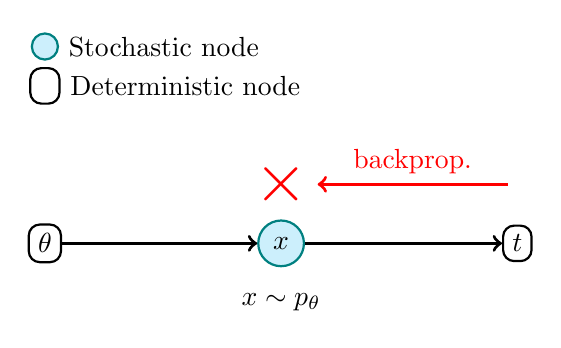
\begin{tikzpicture}
\node[rectangle, rounded corners, thick, draw] (A) at (0,0) {$\theta$};
\node[circle, fill=cyan!20!white, draw=teal, text=black, thick] (B) at (3,0) {$x$};
\node[fill=none]  at (3, -0.75) {$x\sim p_\theta$};

\node[circle, fill=cyan!20!white, draw=teal, text=black, thick] (stoch) at (0,2.5) {};
\node[anchor=west] at (stoch.east) {Stochastic node};
\node[rectangle, rounded corners, thick, draw] (det) at (0,2) {\color{white} t};
\node[anchor=west] at (det.east) {Deterministic node};

\node[rectangle, rounded corners, thick, draw] (C) at (6,0) {$t$};
\node[fill=none, text=red,font=\Huge] (X) at (3, 0.75) {$\times$};
\node[fill=none, text=red] (E) at (6, 0.75) {};

\path[->, very thick] (A) edge node {} (B);
\path[->, very thick] (B) edge node {} (C);
\path[->, red, very thick] (E) edge node[above] {backprop.} (X);
\end{tikzpicture}
\end{minipage}%
\hfill
\begin{minipage}[t]{0.48\textwidth}
\centering
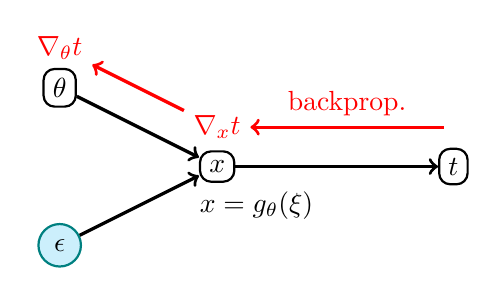
\begin{tikzpicture}
\node[rectangle, rounded corners, thick, draw] (A) at (0,0) {$\theta$};
\node[circle, fill=cyan!20!white, draw=teal, text=black, thick] (Eps) at (0,-2) {$\epsilon$};
\node[rectangle, rounded corners, thick, draw] (B) at (2,-1) {$x$};
\node[fill=none,]  at (2.5,-1.5) {$x=g_\theta(\xi)$};
\node[rectangle, rounded corners, thick, draw] (C) at (5,-1) {$t$};

\node[fill=none, text=red] (X) at (2, -0.5) {$\nabla_x t$};
\node[fill=none, text=red] (E) at (5, -0.5) {};
\node[fill=none, text=red] (S) at (0, 0.5) {$\nabla_\theta t$};

\path[->, very thick] (A) edge node {} (B);
\path[->, very thick] (B) edge node {} (C);
\path[->, very thick] (Eps) edge node {} (B);
\path[->, red, very thick] (E) edge node[above] {backprop.} (X);
\path[->, red, very thick] (X) edge node[above] {} (S);
\end{tikzpicture}
\end{minipage}
\caption{Computational graphs for the objective without the reparameterization trick (left) and with it (right).
By isolating the stochasticity into a separate node, we enable gradient computation with respect to the model parameters.}
\label{fig:repar_trick_visual}
\end{figure}
 Ultimately, we are left with the following SAC algorithm:
 
\begin{algorithm}[H]
\caption{Soft Actor-Critic from \cite{haarnoja2018softactorcriticoffpolicymaximum} (original)}
\label{alg:soft_actor_critic}
\begin{algorithmic}
\STATE \mbox{Initialize parameter vectors $\psi, \bar{\psi}, \theta, \phi$.}
\FOR{each iteration}
	\FOR{each environment step}
	\STATE $a_t \sim \pi_\phi(a_t|s_t)$
	\STATE $s_tp \sim p(s_tp| s_t, a_t)$
	\STATE $\mathcal{D} \leftarrow \mathcal{D} \cup \left\{(s_t, a_t, r(s_t, a_t), s_{t+1})\right\}$
	\ENDFOR
	\FOR{each gradient step}
	\item $\psi \leftarrow \psi - \lambda_V \hat \nabla_\psi J_V(\psi)$
	\STATE $\theta_i \leftarrow \theta_i - \lambda_Q \hat \nabla_{\theta_i} J_Q(\theta_i)$ for $i\in\{1, 2\}$
	\STATE $\phi \leftarrow \phi - \lambda_\phi \hat \nabla_\phi J_\phi(\phi)$
	\STATE $\bar{\psi}\leftarrow \tau \psi + (1-\tau)\bar{\psi}$
	\ENDFOR
\ENDFOR
\end{algorithmic}
\end{algorithm}

\begin{algorithm}[H] 
\caption{Soft Actor-Critic (OpenAI's Spinning Up version \cite{OpenAI_Spinning_UP})} 
\label{alg:SAC} 
\begin{algorithmic} 
\STATE Input: initial policy parameters $\theta$, Q-function parameters $\phi_1$, $\phi_2$, empty replay buffer $\mathcal{D}$ 
\STATE Set target parameters equal to main parameters $\phi_{\text{targ},1} \leftarrow \phi_1$, $\phi_{\text{targ},2} \leftarrow \phi_2$ 
\REPEAT \STATE Observe state $s$ and select action $a \sim \pi_{\theta}(\cdot|s)$ 
\STATE Execute $a$ in the environment 
\STATE Observe next state $s'$, reward $r$, and done signal $d$ to indicate whether $s'$ is terminal 
\STATE Store $(s,a,r,s',d)$ in replay buffer $\mathcal{D}$ 
\STATE If $s'$ is terminal, reset environment state. 
\IF{it's time to update} 
\FOR{$j$ in range(however many updates)} 
\STATE Randomly sample a batch of transitions, $B = \{ (s,a,r,s',d) \}$ from $\mathcal{D}$ 
\STATE Compute targets for the Q functions: \begin{align*} y (r,s',d) &= r + \gamma (1-d) \left(\min_{i=1,2} Q_{\phi_{\text{targ}, i}} (s',
\tilde{a}') - \alpha \log \pi_{\theta}(\tilde{a}'|s')\right), && \tilde{a}' \sim \pi_{\theta}(\cdot|s') \end{align*} 
\STATE Update Q-functions by one step of gradient descent using \begin{align*} & \nabla_{\phi_i} \frac{1}{|B|}\sum_{(s,a,r,s',d) \in B} 
\left( Q_{\phi_i}(s,a) - y(r,s',d) \right)^2 && \text{for } i=1,2 \end{align*} 
\STATE Update policy by one step of gradient ascent using \begin{equation*} \nabla_{\theta} \frac{1}{|B|}\sum_{s \in B} \Big(\min_{i=1,2} 
Q_{\phi_i}(s, \tilde{a}_{\theta}(s)) - \alpha \log \pi_{\theta} \left(\left. \tilde{a}_{\theta}(s) \right| s\right) \Big), \end{equation*} 
where $\tilde{a}_{\theta}(s)$ is a sample from $\pi_{\theta}(\cdot|s)$ which is differentiable wrt $\theta$ via the reparametrization trick. 
\STATE Update target networks with \begin{align*} \phi_{\text{targ},i} &\leftarrow \rho \phi_{\text{targ}, i} + (1-\rho) \phi_i && \text{for } i=1,2 \end{align*} 
\ENDFOR 
\ENDIF 
\UNTIL{convergence} 
\end{algorithmic} 
\end{algorithm}


\subsection{CrossQ}
CrossQ \cite{bhatt2024crossqbatchnormalizationdeep} attempts to introduce batch 
normalization into Q-learning. But what exactly is batch normalization?\newline
Batch normalization is a technique used in deep learning to improve the training of neural 
networks by normalizing the inputs to each layer. It works by adjusting and scaling the 
activations (outputs of neurons). Specifically, it standardizes these activations by 
subtracting the batch mean and dividing by the batch standard deviation, followed by 
scaling and shifting using learnable parameters. Batch normalisation has many benefits such 
as:
\begin{itemize}
    \item Faster Training: It helps the network converge faster by reducing internal 
    covariate shift (i.e., the changing distribution of inputs to each layer during 
    training), making the process more stable.
    
    \item Improved Performance: It often leads to better generalization, reducing 
    overfitting, and improving model performance on unseen data.
    
    \item Allows Higher Learning Rates: Batch normalization enables the use of higher 
    learning rates without causing instability in the training process.
\end{itemize}
However, several people have found that standard batch normalization doesn't work well with 
Q-learning and often makes the learning process more unstable. The issue lies in how the 
Temporal Difference (TD) error is computed in reinforcement learning. So in general the 
loss is defined as 
\begin{align*}
    L_\psi &= \left(\max_{a'}Q_{\psi'}(s_{t+1},a') + r_t - Q_\psi(s_t,a_t)\right)^2 \\
     &= \left(Q_{\psi'}(s_{t+1},\mu_\psi(s)) + r_t - Q_\psi(s_t,a_t)\right)^2 
\end{align*}
%$$ L_\psi = \left(Q_{\psi'}(s_{t+1},a') + r_t - Q_\psi(s_t,a_t)\right)^2$$
where $(s_t,a_t,r_t,s_{t+1})$ are samples from the replay buffer. While $s_t$ and $s_{t+1}$
come from the same distribution, $a_t$ is from the replay buffer, and $a'$ is the action 
predicted by the neural network (which corresponds to the argmax action). This means that
$a_t$ and $a'$ are distributed differently. Since batch normalization requires samples to be independent and identically 
distributed (iid), this discrepancy in distributions introduces the problem. The solution to 
this issue is to concatenate the different state and action batches into a single batch, 
ensuring that all inputs come from the same mixture distribution.
\begin{gather*}
     Q_\psi\left(\begin{bmatrix}
    s_t\\s_{t+1}
\end{bmatrix}, 
\begin{bmatrix}
    a_t\\a'
\end{bmatrix}\right) = \begin{bmatrix}
    q_t\\q_{t+1}
\end{bmatrix} \\
L_\psi = \left(\text{StopGradient}(q_{t+1})+r_t-q_t\right)^2
\end{gather*}
This procedure makes training faster and more efficient overall, as it eliminates the need for a target network.

\subsection{BRO}
The BRO (Bigger, Regularized, Optimistic) paper \cite{nauman2024biggerregularizedoptimisticscaling} shows that scaling model capacity—alongside strong regularization and optimistic 
exploration—can significantly boost sample efficiency in reinforcement learning. Unlike traditional approaches that rely mainly on algorithmic tweaks, BRO leverages large critics and task-specific enhancements to achieve state-of-the-art performances. 

\subsection{Self-Test Questions}
\begin{enumerate}
\sq{ What is the role of the critic in actor-critic methods?}\newline
The critic calculates the TD-Error and tries to learn the value/action-value function

\sq{ Which methods do you know for computing the critic?}\newline
Single sample estimates, N-step returns and Generalized advantage estimation

\sq{Why are off-policy methods more efficient then on-policy methods}\newline
The can use previous collected data to do updates and do not always have to generate new data/discard old data. It also promotes exploring if the samples are chosen randomly from the buffer.

\sq{How can we achieve off-policy RL with continuous actions}\newline
Computing the maximum over actions in the target is a challenge in continuous action spaces. Some solutions are \begin{itemize}
    \item finding the max by doing gradient descent on the Q-network
    \item random shooting: randomly select some actions and take the best performing out of them for calculating the target.
    \item iterative stochastic optimization: same as random shooting but we iteratively update the distribution from which we draw samples to get a better action at the end
    \item learning a neural network to predict the max action
\end{itemize}

\sq{What are the different options to optimize the actor?}\begin{itemize}
    \item stochastic: normal policy gradient where the reward is now changed to be the advantage function
    \item deterministic: learn a deterministic policy that approximates the max operator
    \item variational: regularize RL objective with entropy 
\end{itemize}

\sq{Why do we have a bias in actor critic algorithms and how to fix it?}\newline
The problem is that we use approximators to calculate the targets and since they are bias actor-critics are also bias. That approximator will usually be randomly initialized so it will not give a true estimation of the return, it will be biased towards some random value that was initialized with.

\sq{What type of gradient is DDPG using and why can we not apply the same gradient for the sampled return?}\newline DDPG uses $ \nabla_\theta  \underset{s\sim \mathcal{D}}{\mathbb{E}}[Q_\phi(s,\pi_\theta(s))]
=  \underset{s\sim \mathcal{D}}{\mathbb{E}}\left[ \nabla_a Q_\phi(s,a) \nabla_\theta \pi_\theta(s)|_{a=\pi_\theta(s)}\right]
$

\sq{What is the objective of max-ent reinforcement learning and why is that 
useful?}\newline In entropy-regularized reinforcement learning, the agent gets a bonus 
reward at each time step proportional to the entropy of the policy at that time step. The 
new objective is to maximise this reward. The entropy maximization leads to policies that 
can explore more.

\sq{How to we obtain the policy update in SAC?}
We take the derivative of the Value-Function (Q-Value + Entropy) but with the help 
of the reparametrization trick in order to make the gradient flow through the critic.

\sq{What is the reparametrization trick and when should it be preferred to the likelihood policy gradients?}
It is a trick, in which a sample from $\pi_{\theta}(\cdot|s)$ is drawn by computing a deterministic function of state, policy parameters, and independent noise. The reparametrization trick makes it possible to use the knowledge of the gradient of the Q-function approximation to calculate the gradient of the objective.
\end{enumerate}

\subsection{Resources}
A helpful introduction to actor-critic methods, including the off-policy variants, is provided in Sergey Levine’s CS 285: 
Lecture 6 \cite{CS285,CS285LevineYoutube}. Additionally, the blog posts from OpenAI's Spinning Up series on DDPG, TD3, and SAC 
are excellent resources \cite{OpenAI_Spinning_UP}. For CrossQ, the video \cite{CrossQ_Talk} was particularly informative. For 
BRO, the official website \cite{BRO_Website} offers well-written explanations for those seeking more detailed information.
